\documentclass[14pt]{extarticle}
\usepackage[]{cite}
\usepackage{cmap}
\usepackage[T2A]{fontenc}
\usepackage[utf8]{inputenc}
\usepackage[english, russian]{babel}
\usepackage{amsmath, amsfonts,amssymb,mathrsfs}
\usepackage{graphicx, epsfig}
\usepackage{subfig}
% \usepackage{color}
\usepackage{algorithm}
\usepackage{algorithmic}
\floatname{algorithm}{Алгоритм}
\usepackage{hyperref}
\usepackage{mathrsfs}

\usepackage{wrapfig}
\usepackage{float}
\usepackage{subfloat}
\usepackage{caption}
\usepackage{multirow}
\usepackage{dsfont}
\graphicspath{{./img/}}
% \usepackage{xcolor}
% \usepackage[dvipsnames]{color}
\usepackage[dvipsnames]{xcolor}
\definecolor{mynicegreen}{RGB}{102,252,102}

\newcommand\argmin{\mathop{\arg\min}}
\DeclareMathOperator*{\argmax}{argmax}
\newcommand{\T}{^{\text{\tiny\sffamily\upshape\mdseries T}}}
\newcommand{\hchi}{\hat{\boldsymbol{\chi}}}
\newcommand{\hphi}{\hat{\boldsymbol{\varphi}}}
\newcommand{\bchi}{\boldsymbol{\chi}}
\newcommand{\A}{\mathcal{A}}
\newcommand{\B}{\mathcal{B}}
\newcommand{\x}{\mathbf{x}}
\newcommand{\hx}{\hat{x}}
\newcommand{\hy}{\hat{y}}
\newcommand{\M}{\mathcal{M}}
\newcommand{\N}{\mathcal{N}}
\newcommand{\R}{\mathbb{R}}
\newcommand{\p}{p(\cdot)}
\newcommand{\q}{q(\cdot)}
\newcommand{\uu}{\mathbf{u}}
\newcommand{\vv}{\mathbf{v}}


\renewcommand{\baselinestretch}{1}


\newtheorem{Th}{Теорема}
\newtheorem{Def}{Определение}
\newenvironment{Proof} % имя окружения
    {\par\noindent{\bf Доказательство.}} % команды для \begin
    {\hfill$\scriptstyle\blacksquare$} % команды для \end
\newtheorem{Assumption}{Предположение}
\newtheorem{Corollary}{Следствие}

\textheight=22cm % высота текста
\textwidth=16cm % ширина текста
\oddsidemargin=30pt % отступ от левого края
\evensidemargin=15pt % отступ от правого края
\topmargin=-20mm % отступ от верхнего края
\parindent=24pt % абзацный отступ
\parskip=5pt % интервал между абзацами
\tolerance=2000 % терпимость к "жидким" строкам
\flushbottom % выравнивание высоты страниц
\linespread{1.5}



\begin{document}

\thispagestyle{empty}
\begin{center}
	\linespread{1.3}
    \sc
        ФГАОУВО «Московский физико-технический институт \rm{(национальный исследовательский университет)}»\\
        Физтех-школа аэрокосмических технологий\\
        Кафедра компьютерного моделирования\\[10mm]
    \begin{flushleft}
  \textbf{Направление подготовки:} 01.03.02 Прикладные математика и информатика (бакалавриат) \\
  \textbf{Направленность (профиль) подготовки:} Прикладные математика и информатика \\
  \textbf{Форма обучения:} очная\\[10mm]
  
    \end{flushleft}
    
    {\bf\
		ВЫПУСКНАЯ КВАЛИФИКАЦИОННАЯ РАБОТА \\ «Прогнозирование деградации турбовентиляторных реактивных двигателей с помощью методов глубинного обучения» }\\
		(бакалаврская работа)\\[10mm]
    
\end{center}
		

\hfill\parbox{80mm}{
	\linespread{1.3}
    \begin{flushleft}
    \bf
        Студент:\\
    \rm
        Теслюк Никита Александрович \\[1cm]
    \bf
        Научный руководитель:\\
    \rm
        к.~ф.-м.~н. \\ Аврутский Всеволод Игоревич \\[16mm]
    \end{flushleft}
}
\begin{center}
    Жуковский\\
    2021
\end{center}


\newpage
\linespread{1}
\tableofcontents

\newpage

\section{Введение}
\label{sec:intro}

Многие авиакомпании в последние годы уже получили выгоду от использования искусственного интеллекта (AI --- {\it artificial intelligence}) для мониторинга состояния двигателя (EHM --- {\it engine health monitoring}) и приступили к кампаниям по оптимизации программ, призванным сдерживать расходы и повышать надежность летательных судов. Но, стоит отметить, что относительно немногие преуспели в первых попытках применить ИИ к гораздо более сложным средам обслуживания компонентов и линий, такие как двигатели. Прогностическая сила ИИ может способствовать резкому увеличению прибыльности авиакомпаний за счет устранения сбоев в работе, вызванных техническим обслуживанием, а также повышению безопасности пассажиров.

Анализируя массив исторических данных по техническому обслуживанию воздушных судов и показаний датчиков двигателей, возможна разработка системы, которая позволит прогнозировать в долгосрочной перспективе возможные дефекты по каждому отдельно взятому самолёту. Данная система способна определять вероятность возникновения разных типов дефектов в определенный период в будущем. В случае, если вероятность оказывается выше установленного порога, рекомендуется провести дополнительную проверку воздушного судна и принять должные меры по устранению неполадок.

Исходя из того, что данные, снятые с датчиков, установленных в разных частях двигателя, в большинстве своём являются временными рядами, возникает идея применения современных нейросетевых state-of-the-art подходов глубинного обучения, используемых для работы с последовательностями, таких как рекуррентные нейронные сети и их модификации (RNN, LSTM ). Также в долгосрочной перспективе для повышения точности предсказания возможно использование подходов, базирующихся на технологии Attention \cite{Liu2018DeepRL}, которая широко применяется в области NLP ({\it natural language processing}), а также различных архитектурах типа Transformer \cite{Liu2018DeepRL}.

В данной работе рассматривается применение модели LSTM ({\it Long Short Term Memory}). Главным преимуществом LSTM моделей над классическими RNN является то, что они способны "запоминать" долгосрочные зависимости. Эти модели очень хорошо работают с большим спектром задач и в настоящее время широко используются.

Таким образом, {\bf основной целью} данной работы является предсказание количества оставшихся рабочих циклов двигателей до отказа, с использованием прогнозирующей модели на основе LSTM. Также в работе приведены сравнения рассматриваемой модели с классическими алгоритмами машинного обучения для решения задач регрессии и прогнозирования, таких как случайный лес, градиентный бустинг и др. 

С точки зрения практического исполнения данная работа включает в себя имплементацию модели LSTM. Код, воспроизводящий эксперименты, размещен по \href{https://github.com/teslyuk/bachelors-thesis}{ссылке}.

\newpage

\section{Обзор литературы}
Здесь будет обзор основной литературы, используемой в работе

$1)http://www.machinelearning.ru/wiki/images/a/a1/BayesML-2009-1.pdf \\
2) http://www.machinelearning.ru/wiki/images/e/ed/MOTP14_1.pdf \\
3)http://colah.github.io/posts/2015-08-Understanding-LSTMs/ \\
4)https://www.kaggle.com/behrad3d/nasa-cmaps$

\newpage

\section{Задача прогнозирования}

\subsection{Основные понятия и определения}

Задача прогнозирования исторически возникла при исследовании временных рядов и попытке предсказания их значений через какой-то промежуток времени. 

В классической задаче прогнозирования обучающая выборка представляет собой набор измерений $X = \{\textbf{x}[i]\}_{i = 1}^n$, представляющих собой вектор
вещественнозначных величин $\textbf{x}[i] = \left(x_1[i], . . . , x_d[i]\right)$, $\textbf{x}[i] \in \R^d$ сделанных в определенные моменты времени.

Требуется постросить алгоритм (предиктор), который вернул бы точечную оценку $\{\hat{\textbf{x}}[i]\}_{i = n+1}^{n+q}$ , доверительный интервал $\{\textbf{x}_-[i], \textbf{x}_+[i]\}_{i = n+1}^{n+q}$ или апостериорное распределение $\mathbb{P}(\textbf{x}[n + 1], ... , \textbf{x}[n + q] \: | \: \textbf{x}[1], ... , \textbf{x}[n])$ прогноза на заданную глубину $q$.

\begin{figure}[h]
	\centering
	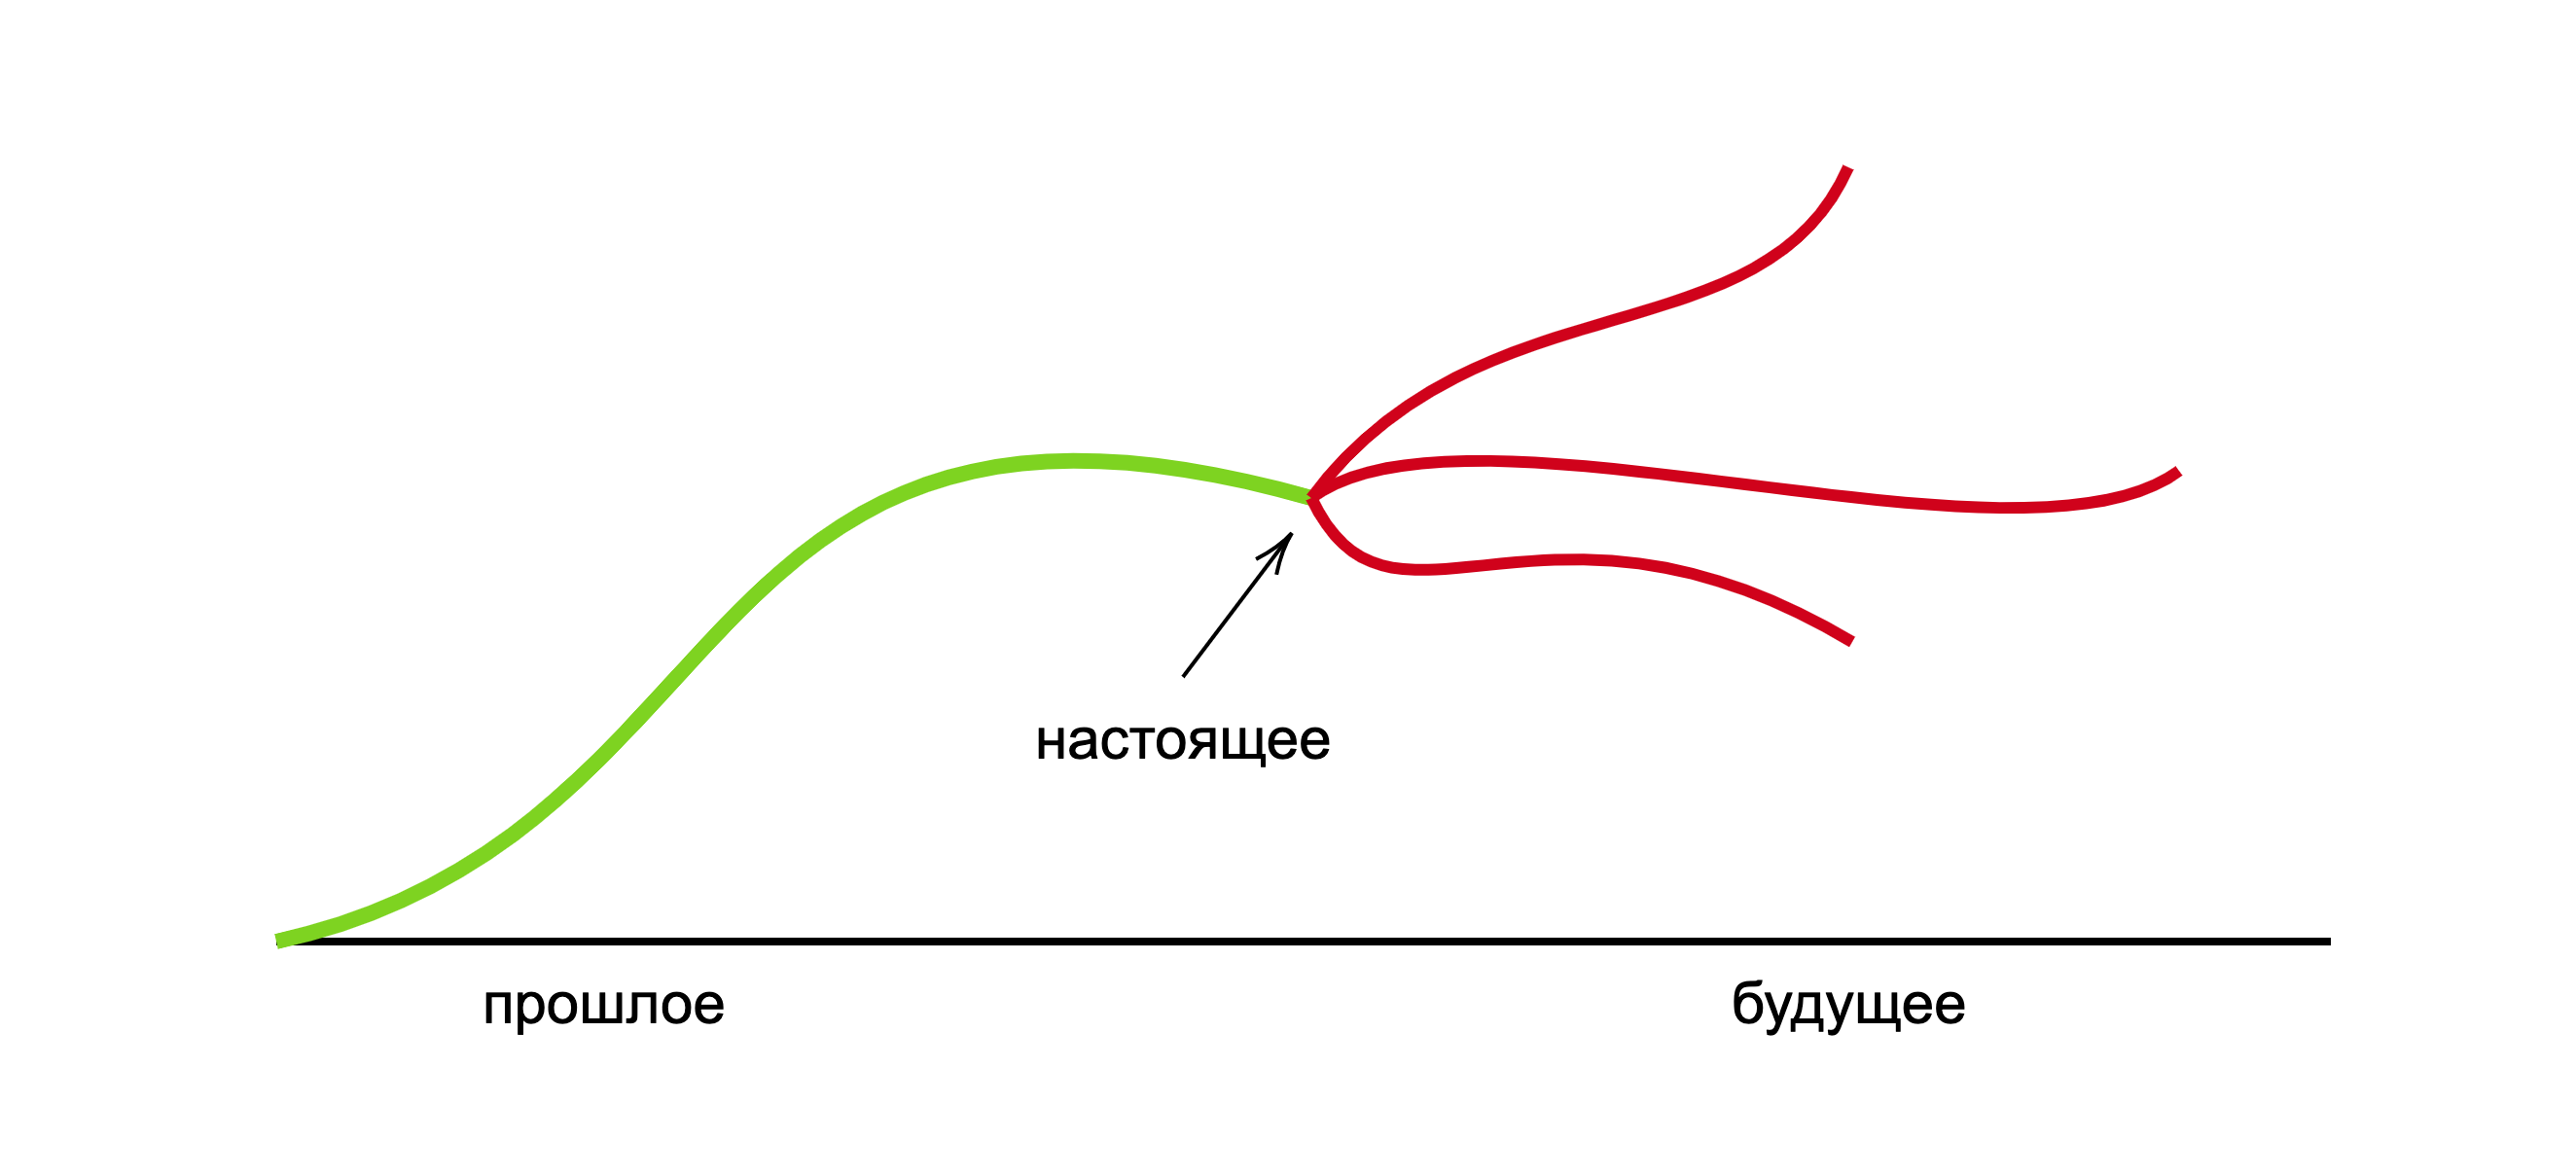
\includegraphics[width=1.0\textwidth]{img/pred_task_diagram_t.png}
	\caption{Иллюстрация прогноза по времени в задачах прогнозирования}
	\label{fig:components}
\end{figure}

Примеры задач прогнозирования:
\begin{itemize}
	
	\item Биржевое дело: прогнозирование биржевых индексов и котировок.
	\item Системы управления: прогноз показателей работы реактора по данным телеметрии.
	\item Экономика: прогноз цен на недвижимость
	\item Демография: прогноз изменения численности различных социальных групп в конкретном ареале
	\item Гидрометеорология: прогноз геомагнитной активности
	
\end{itemize}

\subsection{Постановка задачи}

В рассматриваемой задаче цель состоит в том, чтобы предсказать оставшийся полезный срок службы (RUL --- {\it Remaining Useful Life}) каждого двигателя в наборе тестовых данных. RUL эквивалентно количеству полетов, оставшихся для двигателя после последней точки данных в тестовом наборе данных.

\subsubsection{Описание эксперимента}

Наборы данных состоят из нескольких временных рядов. Данные представляют собой показания датчиков в двигателях. Каждый набор данных далее делится на обучающие и тестовые выборки. Каждый временной ряд относится к определенному отдельно взятому двигателю, т. е. можно считать, что данные относятся к парку двигателей одного и того же типа. Каждый двигатель запускается с разной степенью начального износа и производственными отклонениями, которые неизвестны пользователю. Этот износ и отклонения считаются нормальными, т. е. не считаются дефектом или неисправностью. Есть три рабочих окржунеия (в наборе данных указано, как {\it operational setting}), которые существенно влияют на работу двигателя. Эти настройки также включены в данные. Данные загрязнены шумом датчика.

Двигатель работает должным образом в начале каждого временного ряда и в какой-то момент времени выдает неисправность. В обучающей выборке неисправность нарастает до отказа системы. В тестовом наборе данных временной ряд заканчивается за некоторое время $t$ до сбоя системы. Цель задачи --- спрогнозировать количество оставшихся рабочих циклов до отказа в испытательной установке, то есть количество рабочих циклов после последнего текущего цикла, в которых двигатель будет продолжать работать. Также предоставлен вектор истинных значений оставшегося полезного срока службы (RUL), дабы сверить предсказанные и истинные значения и провести последующий анализ модели. 

\subsubsection{Описание набора данных}

Данные содержат 26 столбцов, содержащих числа, разделенные пробелами. Каждая строка представляет собой массив данных, снятых в течение одного рабочего цикла, каждый столбец --- это отдельная переменная.
\\
\\
Колонки содержат:
\begin{enumerate}
	\item unit number --- номер двигателя
	\item time, in cycles --- время в циклах
	\item operational setting 1 --- режим полёта 1
	\item operational setting 2 --- режим полёта 2
	\item operational setting 3 --- режим полёта 3
	\item sensor measurement 1 --- измерение датчика 1	
	\item sensor measurement 2 --- измерение датчика 2
	\\
	...
	\setcounter{enumi}{25}
	\item sensor measurement 26 --- измерение датчика 26
\end{enumerate}

\subsection{Сведение к задаче глубинного обучения} 

Традиционные подходы к решению задач прогнозирования временных рядов включают в себя регрессионные модели прогнозирования, авторегрессионные модели прогнозирования (ARIMAX, GARCH, ARDLM), модели по выборке максимального подобия (MMSP), модели на основе генетического алгоритма (GA) и множество других. Все они так или иначе устарели или имеют множество своих особенностей и недостатков. 

В последние годы развитие в области искусственного интеллекта и глубинного обучения привело к тому, что новые алгоритмы на основе нейронных сетей в разы превосходят уже существующие традиционные подходы к решению широкого спектра задач. И одним из таких алгоритмов является модель LSTM --- особый вид RNN, способный запоминать долгосрочные зависимости. 

\newpage

\section{LSTM}

\subsection{Проблема долговременных зависимостей}

Одним из преимуществ рекуррентных нейронных сетей (RNN) является то, что они способны сохранять сжатую историческую информацию с предыдущих слоёв сети и подавать её на вход текущему слою, что в свою очередь критически повышает точность используемой модели.

\begin{figure}[h]
	\centering
	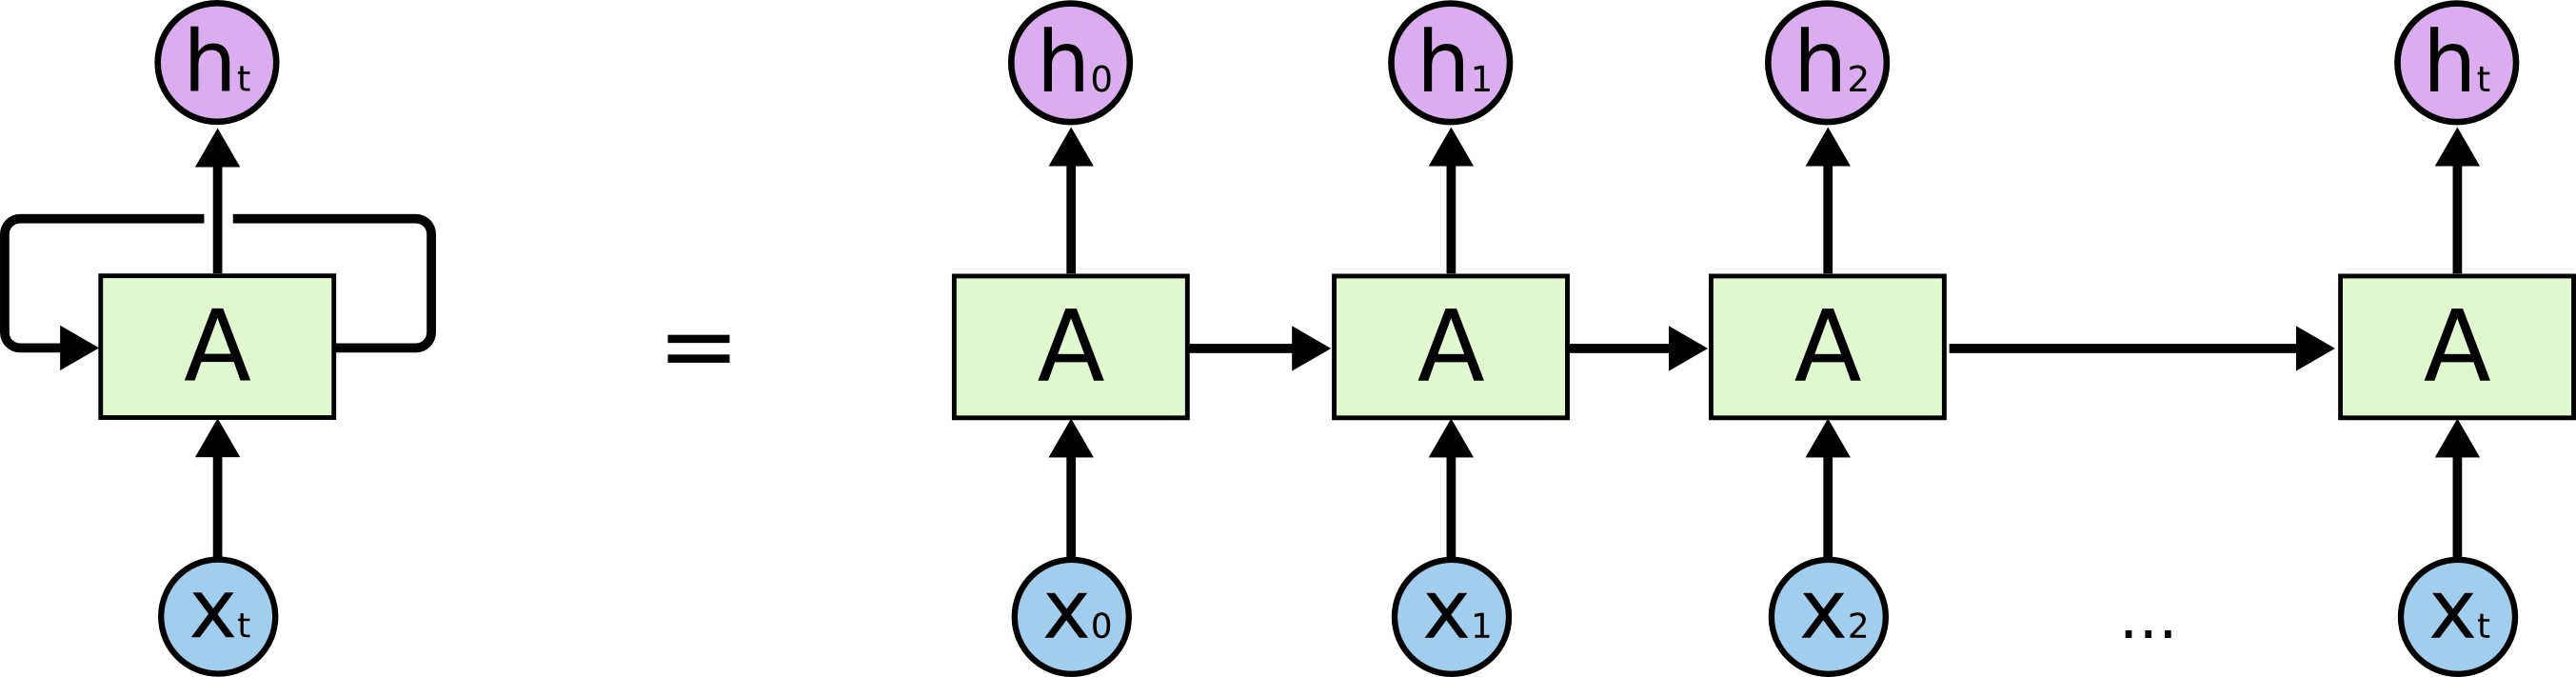
\includegraphics[width=0.85\textwidth]{img/RNN-unrolled.png}
	\caption{Развернутая рекуррентная нейронная сеть. Взято из \cite{Liu2018DeepRL}}
	\label{fig:rnn}
\end{figure}

На приведенной выше диаграмме фрагмент нейронной сети $A$, на вход которой подается некоторый вектор $x_t$ и на выходе извлекатеся вектор скрытого состояния $h_t$. Таким образом рекуррентную нейронную сеть можно рассматривать как несколько копий одной и той же сети, каждая из которых передает сообщение своему преемнику на следующий шаг. Это демонтрирует, что рекуррентные нейронные сети тесно связаны с последовательностями и списками и отлично подходят для работы с данными таких типов. 

Иногда для выполнения какой-либо задачи нам необходима только “недавняя” информация. Например, рассмотрим языковую модель, пытающуюся предсказать следующее слово на основании предыдущих. Если мы хотим предсказать последнее слово в предложении “облака плывут по небу”, достаточно контекста длинной в пару слов по обе стороны от интересующего нас слова; в этом случае довольно очевидно, что последним словом будет “небу”. Видно, что когда дистанция между актуальной информацией и местом, где она понадобилась, невелика, RNN могут обучиться довольно неплохо использую информацию из нескольких предыдущих слоёв.

Но бывают случаи, когда нам необходимо больше контекста. Допустим, мы хотим предсказать последнее слово в тексте “Я вырос во Франции <какой-то текст> Я бегло говорю по-французски”. Ближайший контекст предполагает, что последним словом будет называние языка, но чтобы установить, какого именно языка, нам нужен контекст, указывающий Францию из более отдаленного прошлого. Таким образом, разрыв между актуальной информацией и точкой ее применения может стать очень большим. К сожалению, по мере роста этого расстояния, RNN теряют способность связывать информацию.

В теории проблемы с обработкой долговременных зависимостей у RNN быть не должно. Человек может аккуратно подбирать параметры сети для решения задач различных типов. На практике же обучить RNN этим параметрам кажется невозможным. Эту проблему подробно исследовали Зепп Хохрайтер (Sepp Hochreiter, 1991 \cite{sutton_book}) и Йошуа Бенджио (Yoshua Bengio) с соавторами (1994 \cite{sutton_book}); они нашли неоспоримые причины, по которым это может быть невыполнимой задачей.

\subsection{LSTM сеть}

Долгая краткосрочная память (Long short-term memory; LSTM) --- особая разновидность архитектуры рекуррентных нейронных сетей, способная к обучению долговременным зависимостям. Они были представлены Хохрайтером и Шмидхубером в 1997 \cite{sutton_book} году, а затем усовершенствованы и популяризированы в работах многих других исследователей. Они хорошо справляются с целым рядом разнообразных задач и в настоящее время широко используются в области естественного языка.

LSTM разработаны специально для избежания проблемы долговременной зависимости. Запоминание длинного контекста и сохранение информации на долгие периоды времени --- это их главное свойство. Любая рекуррентная нейронная сеть имеет форму цепи повторяющихся модулей нейронной сети. В обычной RNN структура одного такого модуля очень проста, например, он может представлять собой один слой с функцией активации типа сигмоида или гиперболический тангенс:

% \begin{equation}
$$S(x) = \frac{1}{1 + e^{-x}} = \frac{e^{x}}{e^{x} + 1} = 1 - S(-x),$$ \\
$$f(x) = \tanh{x} = \frac{e^{x} - e^{-x}}{e^{x} + e^{-x}} = \frac{e^{2x} - 1}{e^{2x} + 1}$$
% 	\label{expected_return}
% \end{equation}

В свою очередь LSTM-структура также напоминает цепь, но внутренние модули выглядят иным образом. Вместо одного слоя нейронной сети они содержат целых четыре, и эти слои взаимодействуют особенным образом. 

\begin{figure}[h]
	\centering
	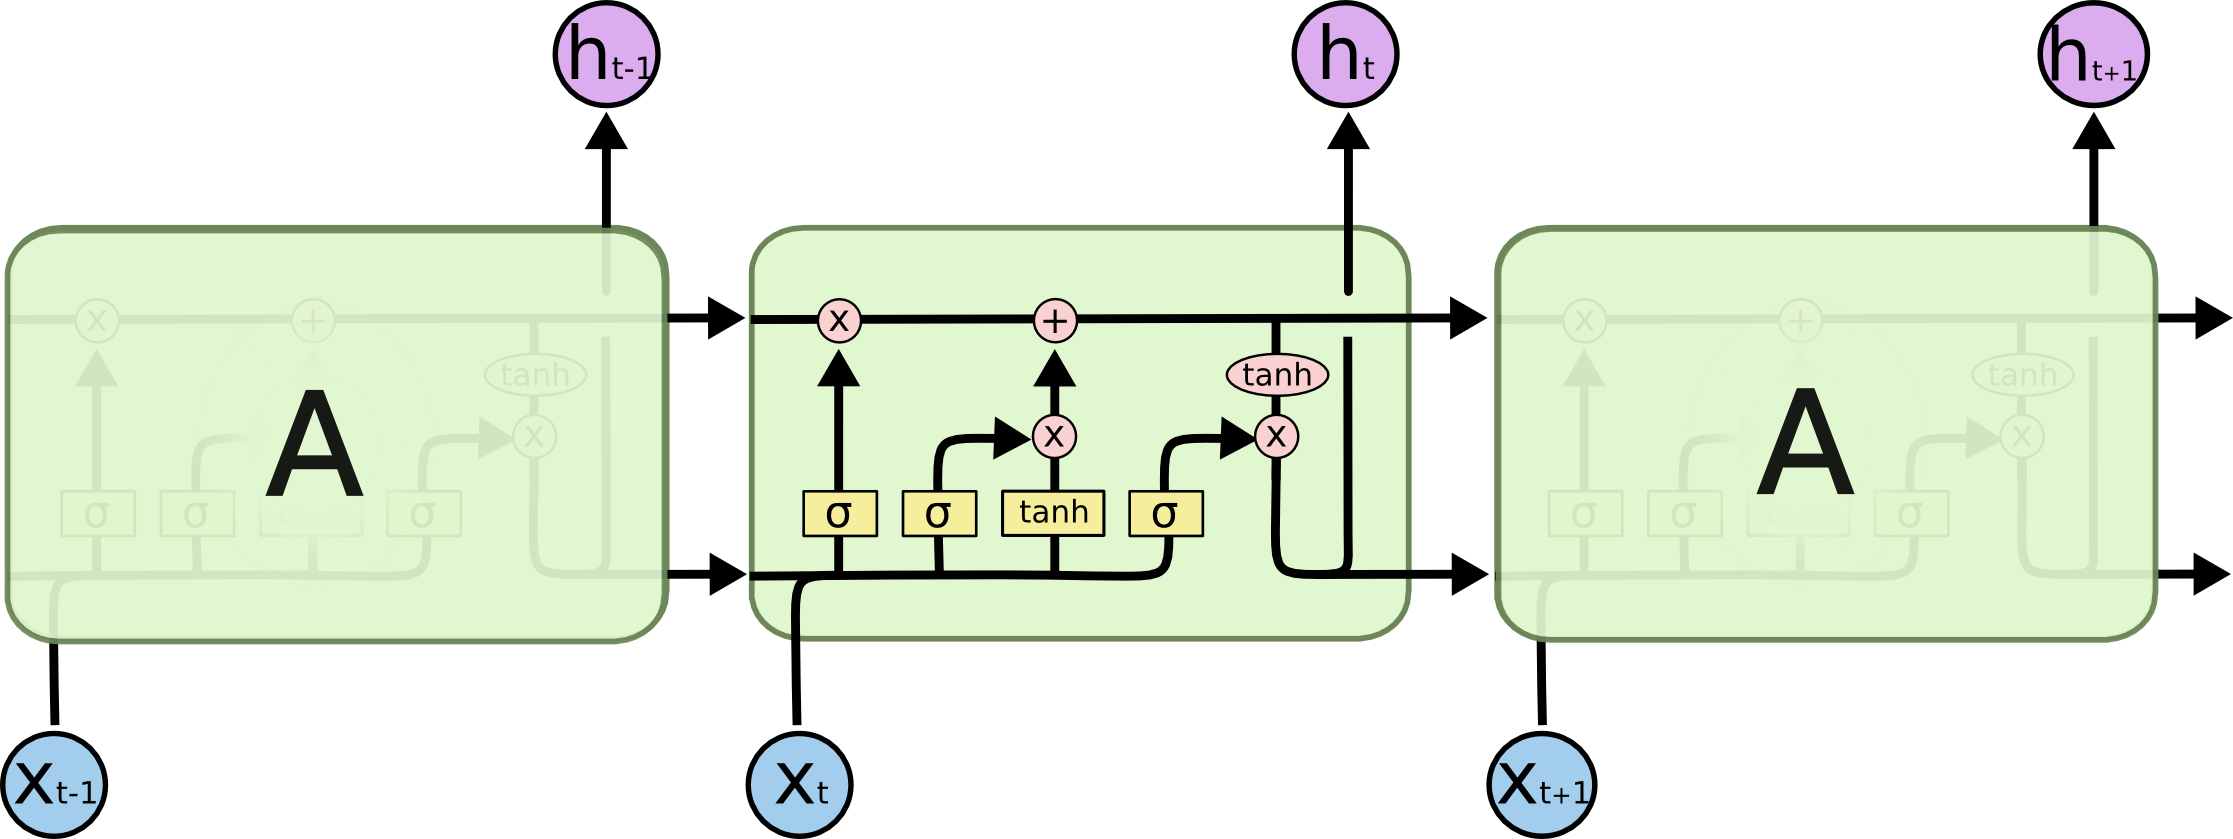
\includegraphics[width=1\textwidth]{img/LSTM-chain.png}
	\caption{Модуль LSTM содержит четыре слоя. Взято из \cite{Liu2018DeepRL}}
	\label{fig:lstm}
\end{figure}

На схеме \ref{fig:lstm} каждая стрелка переносит вектор от выхода одного модуля и подаёт его на вход следующего. Красными кружочками обозначены поточечные операции, такие, как сложение или перемножение векторов. Желтые прямоугольники соответствуют слоям нейронной сети. Сходящиеся стрелки означают объединение, а разветвляющиеся стрелки отвечают за копирование данных и их передачу в другие компоненты сети.

Ключевой концепт LSTM --- состояние ячейки ({\it cell state}) --- горизонтальная линия, проходящая по верхней части схемы. Состояние ячейки проходит напрямую через всю цепочку, участвуя лишь в нескольких линейных преобразованиях. Информация может легко течь по ней, не подвергаясь изменениям. Также LSTM может удалять информацию из состояния ячейки; этот процесс регулируется так называемыми фильтрами ({\it gates}). Фильтры позволяют пропускать информацию на основании некоторых условий. Они состоят из слоя сигмоидальной нейронной сети и операции поточечного умножения. Сигмоидальный слой возвращает числа от нуля до единицы, которые обозначают, какую долю каждого блока информации следует пропустить дальше по сети. Ноль в данном случае означает “не пропускать ничего”, единица --- “пропустить все”. LSTM имеет три таких фильтра, позволяющих защищать и контролировать состояние ячейки.


\subsection{Шаги работы}

\begin{enumerate}

\item
Первый шаг в LSTM --- определить, какую информацию можно выбросить из состояния ячейки. Это решение принимает слой сигмоиды, называемый “слоем фильтра забывания” (forget gate layer). Он смотрит на $h_{t-1}$  и $x_t$ и возвращает число от 0 до 1 для каждого числа из состояния ячейки $C_{t-1}$. Единица означает “полностью сохранить”, а ноль – “полностью выбросить”.

\begin{figure}[h]
	\centering
	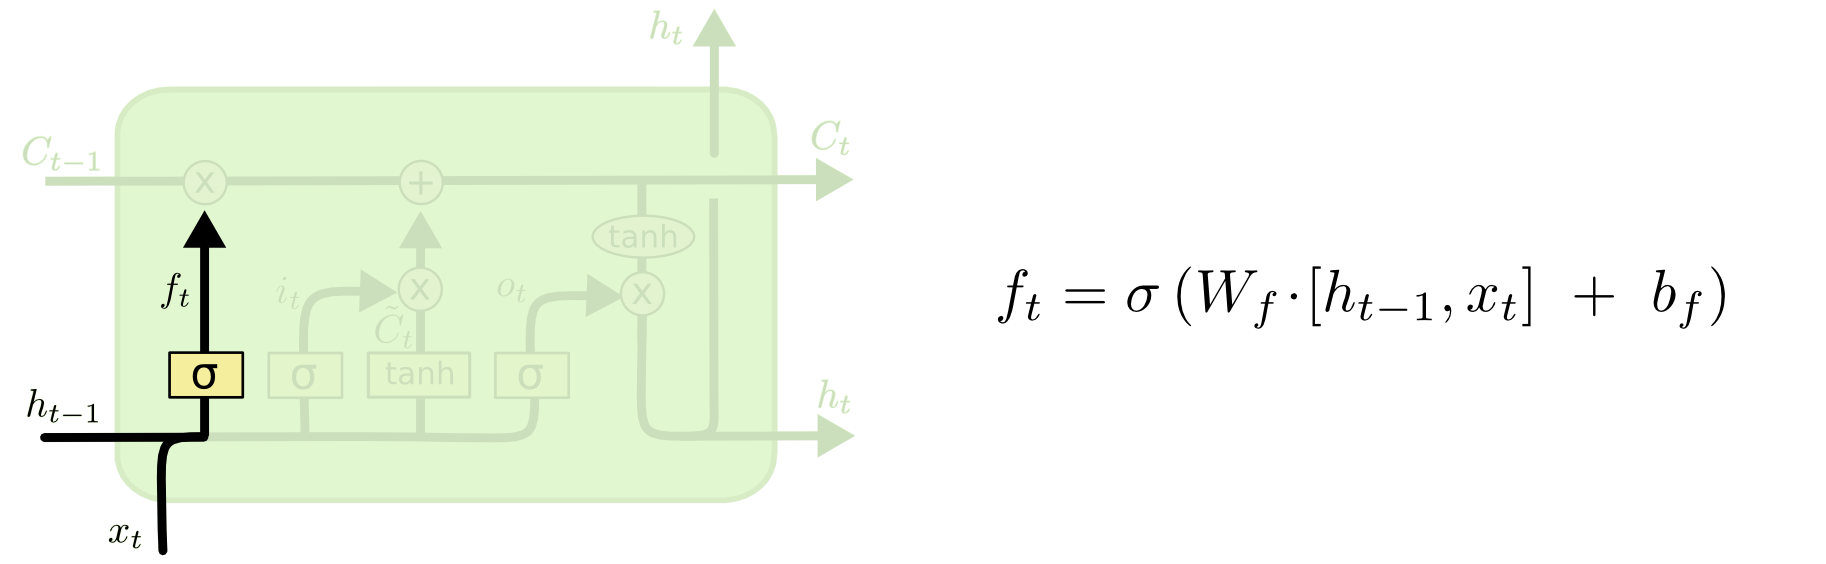
\includegraphics[width=1\textwidth]{img/LSTM-step_1.png}
	\caption{Первый шаг. Взято из \cite{Liu2018DeepRL}}
	\label{fig:lstm-s1}
\end{figure}

\item
Второй шаг --- решить, какого рода новая информация будет храниться в состоянии ячейки. Сначала “слой входного фильтра” ({\it input layer gate}) определяет, какие значения следует обновить. Затем tanh-слой строит вектор новых значений-кандидатов $\widetilde{C_t}$, которые можно добавить в состояние ячейки.

\begin{figure}[h]
	\centering
	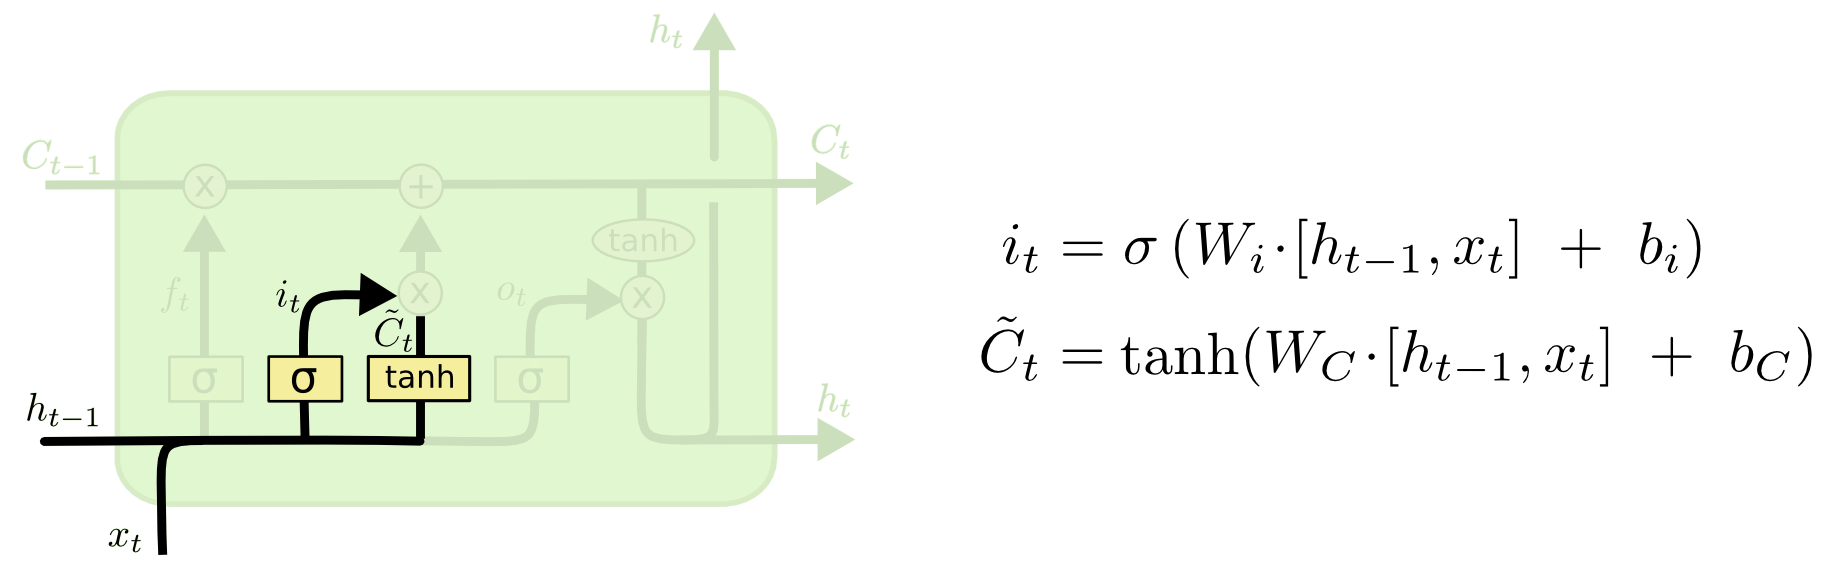
\includegraphics[width=1\textwidth]{img/LSTM_step_2.png}
	\caption{Второй шаг. Взято из \cite{Liu2018DeepRL}}
	\label{fig:lstm-s2}
\end{figure}

\item
Третьим шагом требуется заменить старое состояние ячейки $C_{t - 1}$  на новое $C_t$. Для этого нужно умножить старое состояние на $f_t$, тем самым забывая ненужную информацию. Затем прибавить $i_t * \widetilde{C_t}$, чтобы получить информацию о том насколько нужно обновить каждое из значений нового состояния.

\begin{figure}[h]
	\centering
	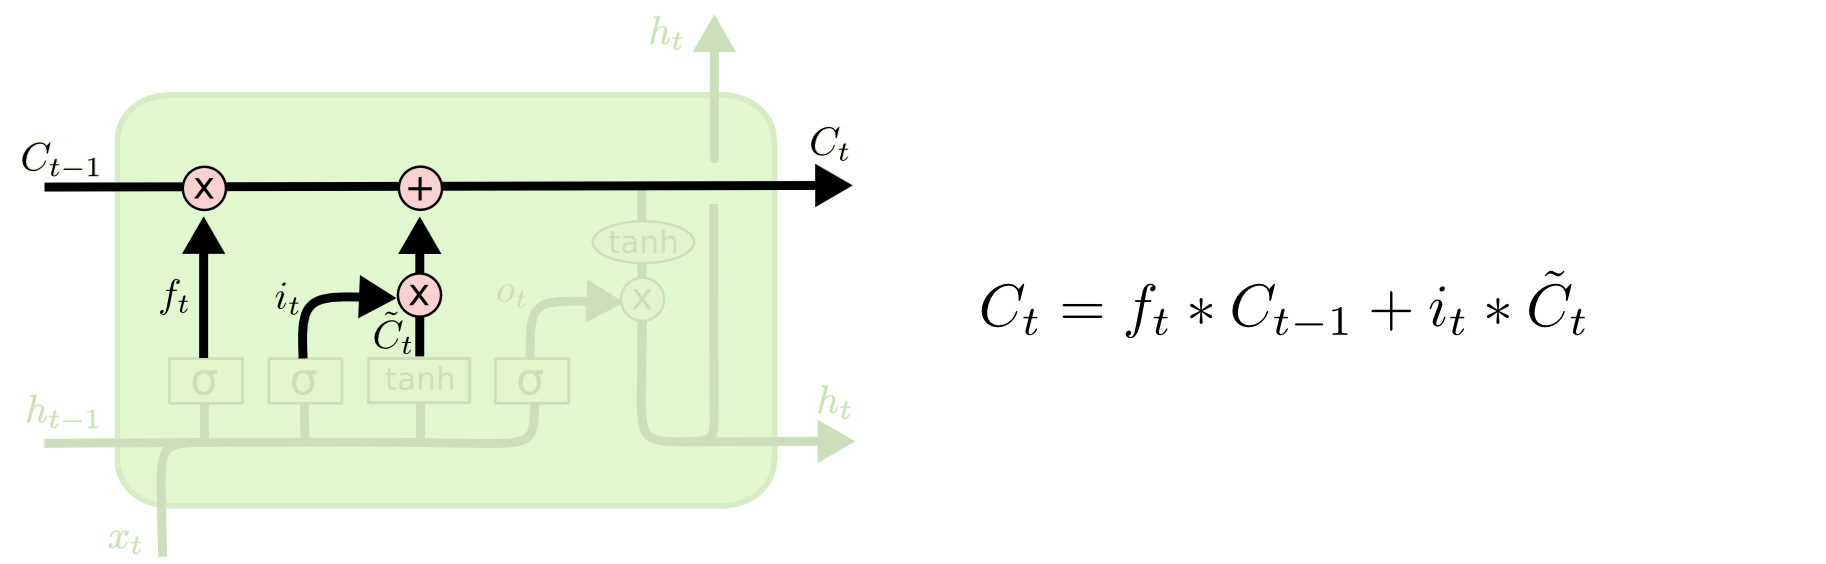
\includegraphics[width=1\textwidth]{img/LSTM_step_3.png}
	\caption{Третий шаг. Взято из \cite{Liu2018DeepRL}}
	\label{fig:lstm-s3}
\end{figure}

\item
На последнем шаге нужно решить, какая информация должна быть на выходе. Выходные данные будут основаны на текущем состоянии ячейки. Сначала требуется применить слой сигмоиды, который определяет, какую информацию из состояния ячейки мы будем выводить. Затем применяется tanh-слой, чтобы получить на выходе значения из диапазона от -1 до 1, которые перемножаются с выходными значениями слоя сигмоиды, что позволяет выводить только требуемую информацию.

\begin{figure}[h]
	\centering
	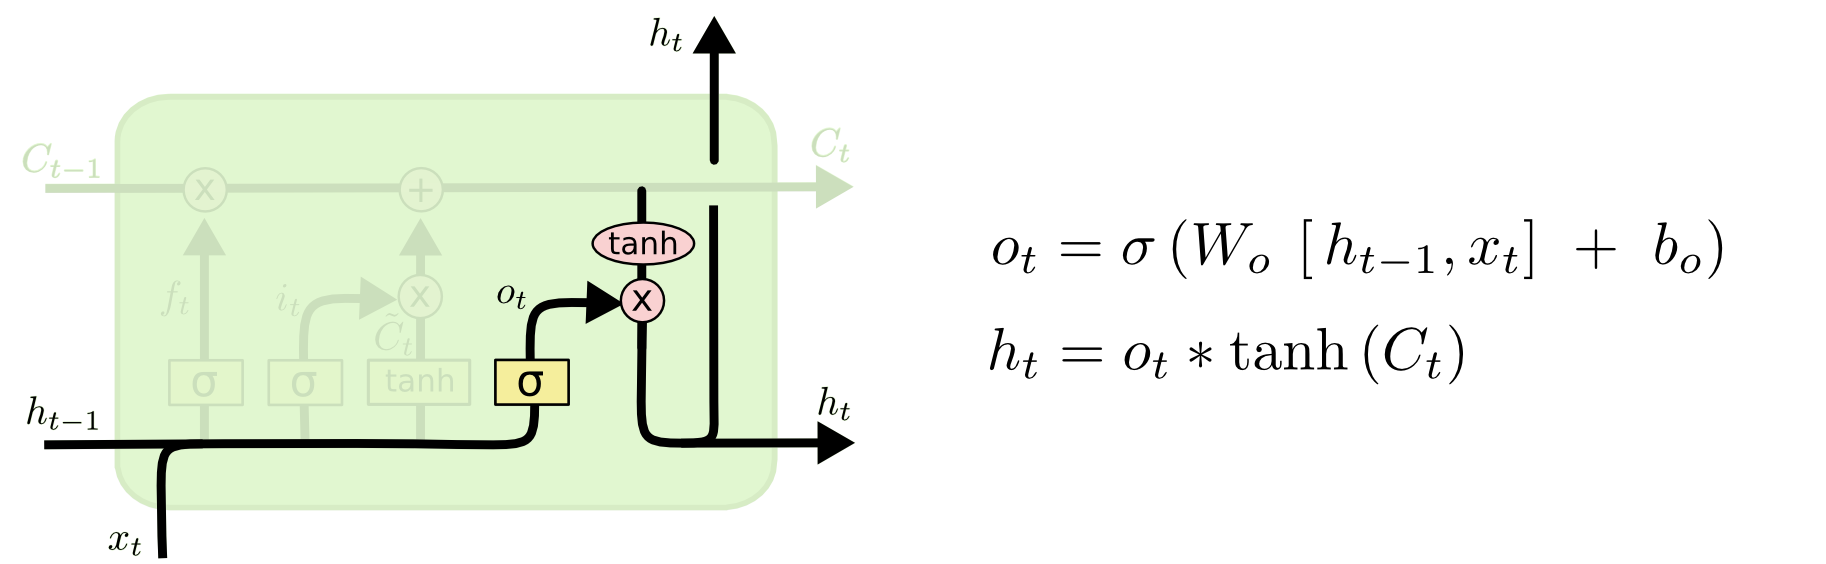
\includegraphics[width=1\textwidth]{img/LSTM_step_4.png}
	\caption{Четвёртый шаг. Взято из \cite{Liu2018DeepRL}}
	\label{fig:lstm-s4}
\end{figure}

\end{enumerate}

\newpage

\section{Вычислительный эксперимент}

\subsection{Предобработка данных}

Для экспериментов был выбран набор данных с сайта NASA за авторством A. Saxena, K. Goebel, D. Simon, and N. Eklund (2008) \cite{ML_1M}, содержащий:

\begin{itemize}
    \item $\sim$20,000 строк в тренировочной выборке, 100 уникальных id двигателей;
    \item $\sim$13,000 строк в тестовой выборке, 100 уникальных id двигателей;
    \item 100 строк --- ground truth метки
\end{itemize}

Из данных были удалены скореллированные признаки (> 80\% корелляции), как из тренировочной выборки, так и из тестовой выборки. Далее, оба набора данных были очищены от шума, пробелы в колонках были заменены на усреднённые показания по конкретно рассматриваемому признаку. Также была произведена нормировка признаков с помощью MinMaxScaler:

% \begin{equation}
$$x_{scaled} = \frac{x - x_{min}}{x_{max} - x_{min}}$$ 
% \end{equation}




\subsection{Обучение модели}

В качестве модели используется глубокуя LSTM сеть. На первом слое --- LSTM со 100 единицами ({\it units --- размерность выходного пространства}), за которым следует еще один слой LSTM с 50 единицами. Dropout, равный $0.2$ применяется после каждого слоя LSTM для улучшения точности модели, а также во избежание переобучения. Последний слой --- это полносвязная сеть с активацией типа сигмоида и одномерным выходом. Количество тренируемых параметров $\sim$80,000. Архитектура нейронной сети представлена на схеме \ref{fig:lstm-arch}:

\begin{figure}[h]
	\centering
	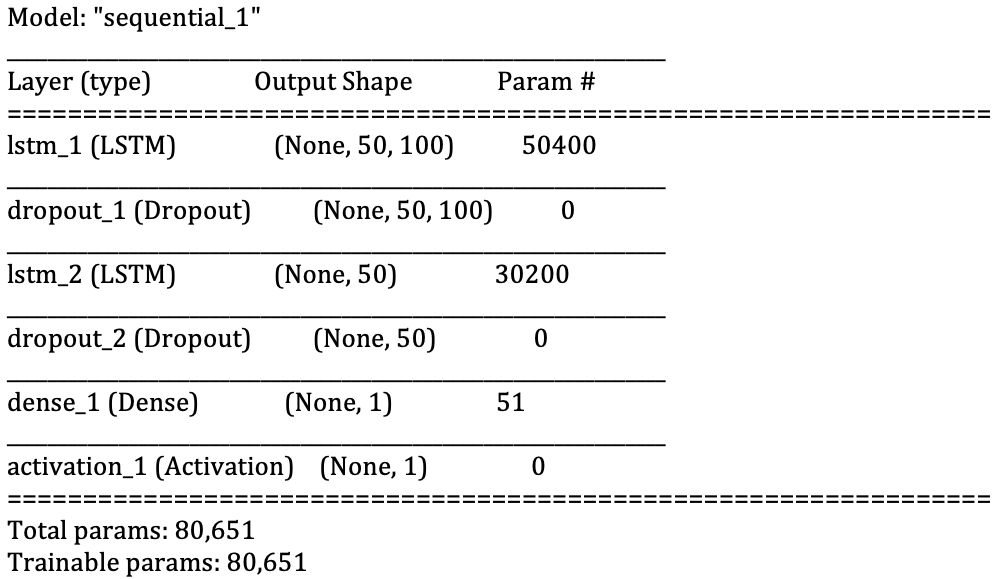
\includegraphics[width=0.95\textwidth]{img/nn_structure2.png}
	\caption{Архитектура нейронной сети.}
	\label{fig:lstm-arch}
\end{figure}

Обучение производится на 80\% тренировочной выборки. Остальные 20\% данных в тренировочном датасете отложены для валидации модели. Дополнительно, используется механизм Early Stopping --- остановка обучения нейронной сети при выходе ошибки на плато либо при её систематическом увеличении для сохранения оптимальных параметров. Сеть обучается на протяжении 100 эпох ({\it epoch} --- полный цикл обучения). Размер батча ({\it batch --- кусок данных для обучения на конкретном шаге}) равен 200. В качестве метрик используются MAE ({\it mean absolute error}) и коэффициент детерминации $R^2$. Все описанные параметры являются оптимальными и были получены эксперементальным путём в ходе процедуры Grid Search.

Ниже приведён алгоритм обучения модели:

\begin{algorithm}[H]
	\caption{{Процедура обучения}}
	
	\begin{algorithmic}[1]
		\STATE Разбить тренировочную выборку на батчи $X_{batch} = \{\textbf{x}[i]\}_{i = 1}^{n}$ по 200 элементов
		\FOR{$\text{t}=1,\dots num\_epochs$}
		\STATE Подать на вход последовательность из батча в виде вектора
		\STATE Вычислить предсказание на текущем шаге
		\STATE Сделать шаг градиентной оптимизации
		\STATE Перейти на следующую итерацию
		\ENDFOR
		
		\hspace*{\algorithmicindent} \textbf{Выход:} усредненные значения остаточного числа циклов работы двигателя за $n$ батчей
	\end{algorithmic}
\end{algorithm}

\subsection{Валидация модели}

Так как рассматриваемые данные представляют собой временные ряды, то они упорядочены относительно неслучайных моментов времени, а следовательно, в отличие от случайных выборок, могут содержать в себе дополнительную важную для обучения информацию, которую нельзя терять. Поэтому стандартные техники валидации в этом случае являются непригодными для использования. Таким образом, в процессе валидации пришлось использовать более специфический способ для оптимизации параметров, так называемый {\it cross-validation on a rolling basis} или кросс-валидация на скользящем окне. 

\begin{figure}[h]
	\centering
	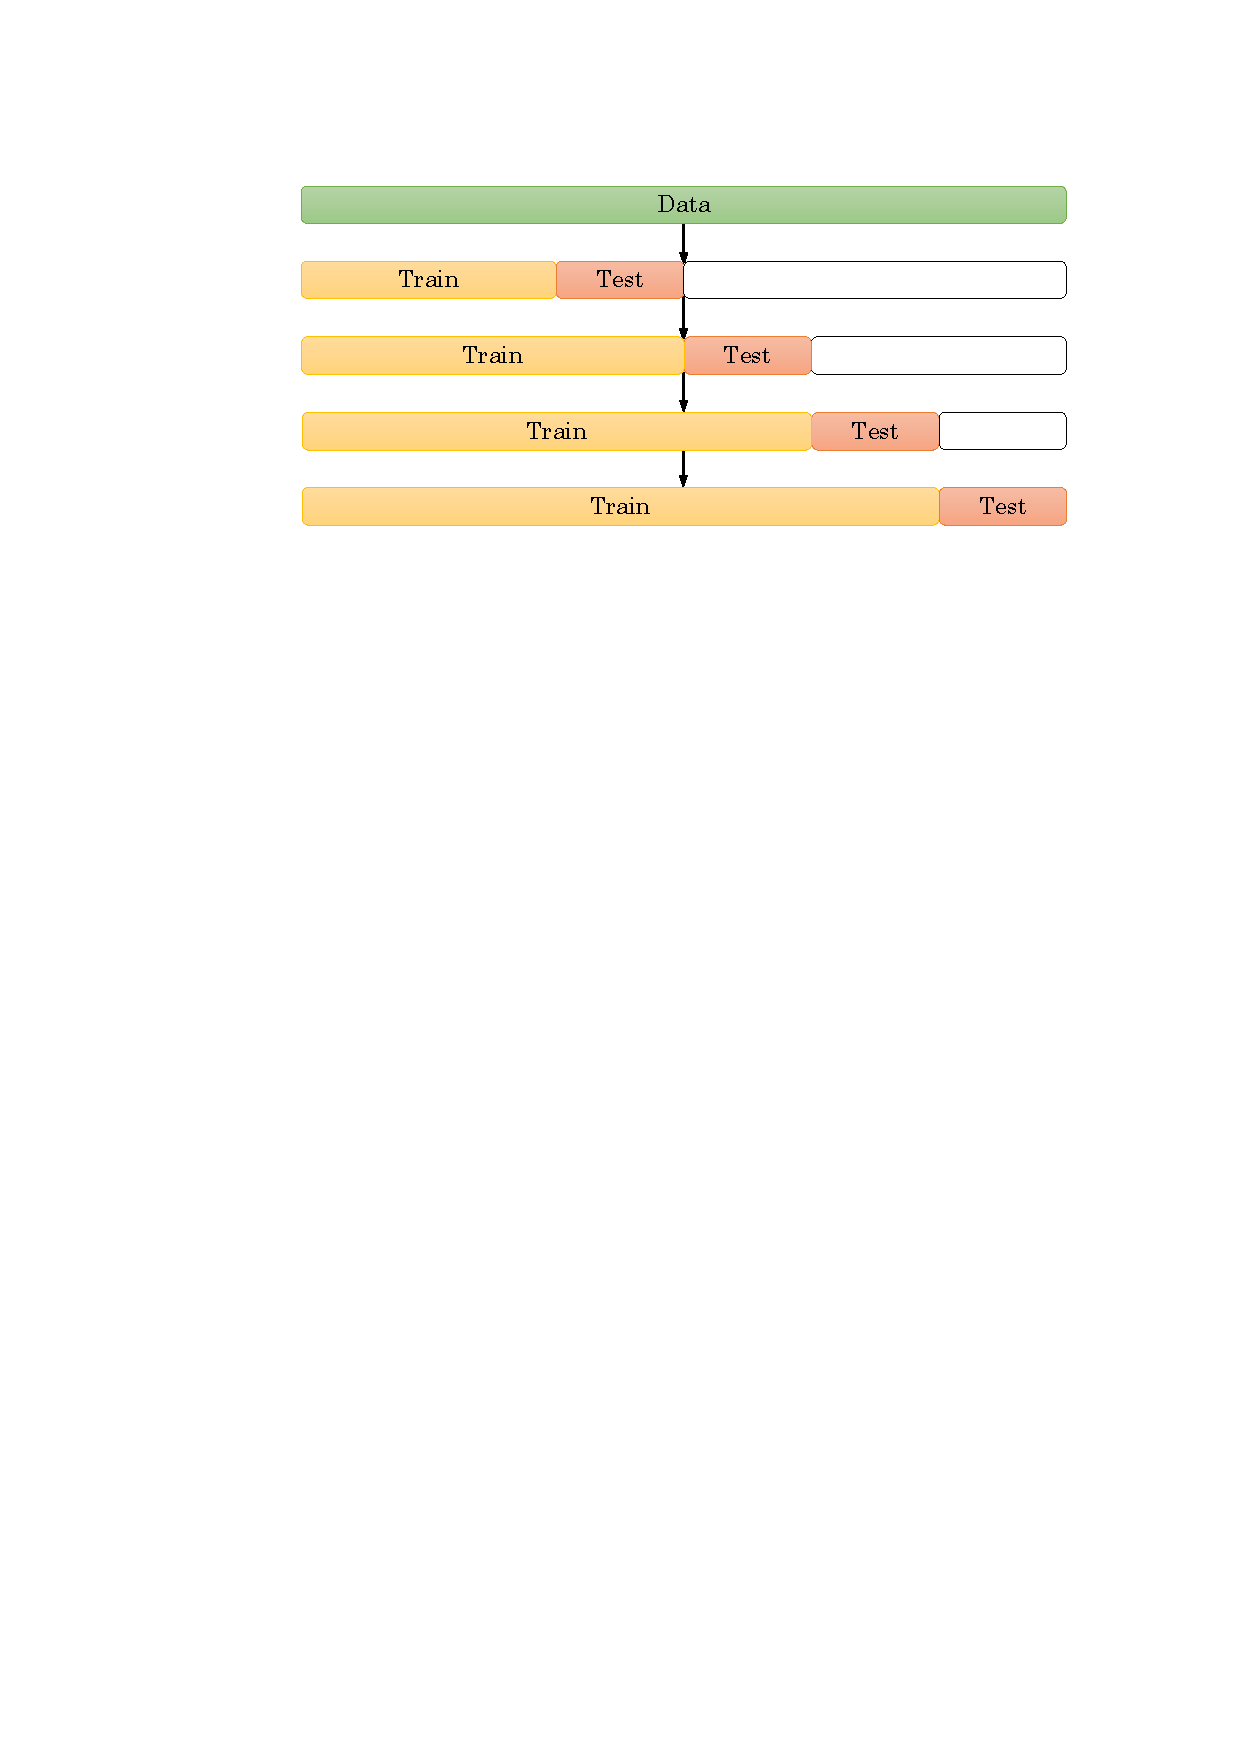
\includegraphics[width=0.95\textwidth]{img/sliding_window_val.pdf}
	\caption{Схема валидации.}
	\label{fig:sliding_window}
\end{figure}

Суть такого подхода состоит в том, что сначала модель обучается на небольшом отрезке временного ряда, от начала до некоторого момета времени $t$, затем делается прогноз на $t + n$  шагов вперед и считается ошибка. Далее обучающая выборка расширяется до  значения $t + n$ и прогнозируется с $t + n$ до $t + 2n$. Так продолжает двигаться валидационный отрезок ряда до тех пор, пока не упирается в последнее доступное наблюдение. В итоге получится столько фолдов --- групп данных, сколько $n$ уместится в промежуток между изначальным обучающим отрезком и всей длиной рассматриваемого ряда.

\subsection{Проверка на тестовых данных}



\subsection{Результаты}

В ходе обучения критерии качества измерялись двумя способами. 
Раз в 10000 шагов измерялось качество на всей тестовой выборкее, раз в 100 шагов --- на одном случайно выбранном изначально пользователе.

\begin{figure}[H]
	\begin{minipage}[b]{0.49\textwidth}
		\centering
		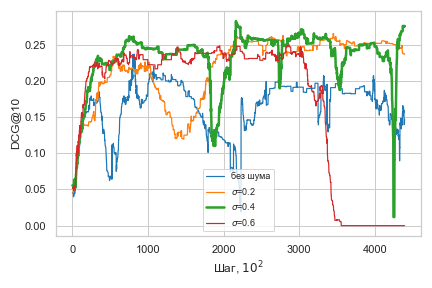
\includegraphics[scale=0.55]{img/curve_dcg.png}
	\caption{Кривая обучения DCG@10 для одного пользователя}
	\label{fig:hit_curve}
	\end{minipage}
	\hfill
	\begin{minipage}[b]{0.49\textwidth}
		\centering
		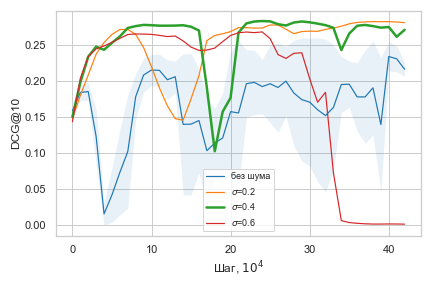
\includegraphics[scale=0.55]{img/curve_dcg_all_.png}
	\caption{Кривая обучения DCG@10 для всех пользователей}
	\label{fig:hit_curve}
		
	\end{minipage}
\end{figure}

Синим затемнением на графике отмечено стандартное отклонение по трём запускам модели без шума.

\begin{figure}[H]
	\begin{minipage}[b]{0.49\textwidth}
		\centering
		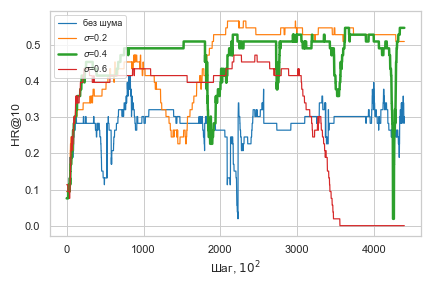
\includegraphics[scale=0.55]{img/curve_hit.png}
	\caption{Кривая обучения HR@10 для одного пользователя}  
	\label{fig:hit_curve}
	\end{minipage}
	\hfill
	\begin{minipage}[b]{0.49\textwidth}
		\centering
		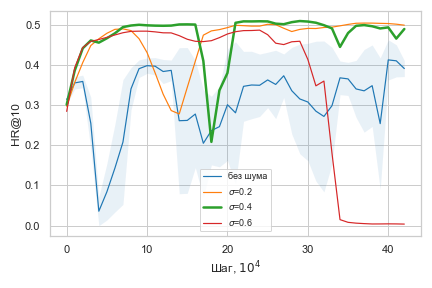
\includegraphics[scale=0.55]{img/curve_hit_all_.png}
	\caption{Кривая обучения HR@10 для всех пользователей}
	\label{fig:hit_curve}
	\end{minipage}
\end{figure}


Для итогового вычисления качества модели использовались наилучшие веса из истории оценивания по всем пользователям. Результаты представлены в таблице \ref{Tab:results}

\begin{center}
	\begin{table}[h]
		\centering
		%\begin{tabular}{l|l|l|l}
		\begin{tabular}{ccc}
			\hline Модель & DCG@10 &  HR@10 \\
			\hline $\sigma = 0.6$ & 0.268  & 0.487\\
			$\pmb{\sigma = 0.4}$  & {\bf 0.282} & {\bf 0.509} \\
			$\sigma$ = 0.2 & {\bf 0.282}  & 0.504\\
		    без шума & 0.254 & 0.454 \\
			Случайные рекомендации & $\sim 0.05$ & $\sim 0.1$   \\
			\hline 
		\end{tabular}
		\caption{Сравнение разных вариантов шума}
		\label{Tab:results}
	\end{table}
\end{center}

Видно, что использование шума повышает как итоговые критерии качества, так и их промежуточные значения в процессе обучения.

\newpage

\section{Заключение}

\subsection{Итоги работы}

В рамках проведенного исследования была достигнута поставленная цель и решены
сформулированные в начале исследования задачи. На защиту выносятся следующие результаты:
\begin{enumerate}
\item Разработана модель ранжирования рекомендаций на основе алгоритма обучения с подкреплением актор-критик с использованием стохастических процессов Орнштейна~---~Уленбека
\item Показано, что оптимизация дисперсии процессов Орнштейна~---~Уленбека улучшает качество рекомендаций по~критериям DCG и HR.
\item Показано, что детерминированные предсказания затрудняют исследование среды агентом.
\end{enumerate}

\subsection{Дальнейшие исследования}

Рассматриваются следующие возможные варианты развития данной работы:

\begin{enumerate}
\item Изучить подходы к построению состояний среды.

\item Сравнить рассмотренный в данной работе метод с другими упомянутыми перспективными алгоритмами, такими как trulyPPO \cite{trulyPPO}.
\item Исследовать более сложные постановки задач рекомендательного моделирования, включая многошаговые рекомендательные сценарии, где на каждой итерации происходит переформулировка или уточнение запроса. Такая постановка задачи близка к разведочному поиску. Обычно разведочный поиск включает в себя несколько итераций поисковых запросов, а также используется в случаях, когда пользователь не имеет четкого запроса или представления о требуемом результате поиска. Цель такого поиска — не только найти информацию, точно соответствующую запросу, но и осознать, изучить новую тему. Обучение с подкреплением --- подходящий метод для решения такой задачи. Таким образом, данное исследование может быть продолжено не только в рамках рекомендательного моделирования, но и в рамках алгоритмов поиска текстовых документов.

\end{enumerate}

Также в дальнейшем планируется перейти на использование фреймворка Catalyst (включен в Pytorch Ecosystem) \cite{catalyst}.

\newpage


%%%%%%%%%%%%%%%%%%%%%%%%%%%%%%%%%%%%%%%%%%%%%%%%%%%%%%%%%%%%%%%%%%%%%%%%%
\newpage
\addcontentsline{toc}{section}{\protect\numberline{}Список литературы}
\bibliographystyle{ugost2008}
\bibliography{recsys_rl}
\nocite{*}







\end{document} 